\documentclass{article}

\usepackage[scale=0.7]{geometry}
\usepackage{hyperref, tablefootnote, color, graphicx, float, caption, subcaption}
\usepackage{titlesec}
\graphicspath{{../final_presentation/figs/}}
\setcounter{secnumdepth}{4}

\titleformat{\paragraph}
{\normalfont\normalsize\bfseries}{\theparagraph}{1em}{}
\titlespacing*{\paragraph}
{0pt}{3.25ex plus 1ex minus .2ex}{1.5ex plus .2ex}

\newcommand{\todo}[1]{\textcolor{red}{\textbf{[#1]}}}

\title{PhotoHunter: A Citizen-Scientist Game with User-in-the-loop
  Data Confirmation for Collecting Computer Vision Datasets of
  Geo-tagged Imagery through Crowd-Sourcing Data Collection; Abstracting
  Research using an Interactive, Game-based Mobile Application for Large
  Dataset Creation
  \footnote{Project location:
    \url{https://github.com/QuesoTech/PhotoHunter}
  }
}

\author{
	Ryan Baltenberger \and
	Aaron Bradshaw \and
	Connor Greenwell \and
	J.\ David Smith \and
	Scott Workman\footnote{Customer}
}

\date{}

\begin{document}

\maketitle

\begin{center}
  \textit{CS 499 --- Senior Design, University of Kentucky, \today}
\end{center}

\begin{abstract}
  The PhotoHunter project is a system intended to simplify the creation of
  datasets for computer vision research by the process of "gamification". The
  system is composed of two mobile applications and a web interface. The web
  interface allows researchers to specify a set of images based on their needs.
  Based on these specifications, the first mobile application generates a list of
  descriptions for photos. Users then capture photos matching these descriptions
  and submit them in a scavenger-hunt style game. The second mobile application
  uses the submitted photos to quiz users. The players are briefly shown the
  images and then asked to label them. Based on the most-commonly provided
  answer, the correct label for the image can be determined. The labelled images
  are then provided to the researchers that requested the dataset. The system
  provides entertainment for users and useful datasets for researchers.
\end{abstract}

\section{Disclaimer}
This project has been designed and implemented as a part of the requirements
for CS-499 Senior Design Project for Spring 2014 semester.  While the authors
make every effort to deliver a high quality product, we do not guarantee that
our products are free from defects.  Our software is provided "as is," and you
use the software at your own risk.

We make no warranties as to performance, merchantability, fitness for a
particular purpose, or any other warranties whether expressed or implied.

No oral or written communication from or information provided by the authors or
the University of Kentucky shall create a warranty.

Under no circumstances shall the authors or the University of Kentucky be
liable for direct, indirect, special, incidental, or consequential damages
resulting from the use, misuse, or inability to use this software, even if the
authors or the University of Kentucky have been advised of the possibility of
such damages.


\section{Introduction}

One of the largest roadblocks to successful computer vision is the difficulty of
acquiring large quantities of accurate ground truth data for a given problem
statement. Traditionally, this task has been relegated to under-paid and over-worked
underclassmen or new graduate students. This technique has produced some of the
most famous datasets in the field (Caltech-101, Caltech-256). However, the size of
these datasets no longer supports current machine learning research. Recently,
many researchers have opted to use Amazon Mechanical Turk to create and verify their
datasets. However, due to the nature of outsourcing tasks to those motivated to
perform them quickly and thoughtlessly using AMT comes at a hefty financial and
accuracy cost.

Many researchers have experimented with this and other forms of ``citizen science''
for data collection and verification. Outsoucing data collection tasks is especially
valuable for when it is impossible, financially or practically, for researchers to
collect their data themselves (ornithologists figured this out many years ago).

We propose a ``citizen science'' system for collecting large, verified sets of images
for computer vision research by ``game-ifying'' the interface. Rather than instruct
users to ``collect imagery and atmospheric data around trees in urban areas'', they
will be on a {\em scavenger hunt} taking pictures to try and beat their friends.
Similarly, rather than asking users to ``verify that the image is of a dog'', they
will be playing a quick recall game wherein they're asked what a picture was of after
a split second.

To this end we have created a three part software suite, titled {\em PhotoHunter}
which consists of the following:
\begin{description}
	\item[PhotoHunter] A photo scanvenger hunt app for collecting images
	\item[QuickPic] Quick response game for collecting labels for images
	\item[Researcher Interface] For requesting and viewing datasets
\end{description}

Our customer for this project is a graduate student with the Computer Science
Department, Scott Workman. We expect the users of our product suite would be
two-fold: researchers interested in collecting datasets this way; and the general
mobile-gaming public.

\section{Product Specifications}

\subsection{Environment}

\subsubsection{Web Browsers}
The web interface for the PhotoHunter Project will be compatible with the
versions of Google Chrome and Mozilla Firefox that are available on April 1,
2015. This interface will also employ a responsive design to accommodate users
visiting on a mobile device's browser.

\subsubsection{Mobile Application}
The two mobile applications for the PhotoHunter Project will be developed with
cross-platform tool, allowing the applications to be deployed to Android
version 4.4.2 (Kit-Kat).

\subsection{Architecture}

\subsubsection{Overview}
The components of the PhotoHunter Project will each utilize the same database
for different purposes.

\subsubsection{Web Interface}
The web interface will allow researchers to specify an image dataset based on
their needs. This specification is then used as a topic for the PhotoHunter
mobile application. Researchers may also use the web interface retrieve their
finalized dataset after the images have been labeled by the QuickPic mobile
application.

\subsubsection{PhotoHunter}
This mobile application generates lists based on the topics provided by
researchers through the web interface. Users playing the PhotoHunter game
capture photos matching the topics in the list. These photos are uploaded to
the overall system's database for use in dataset generation.

\subsubsection{QuickPic}
This mobile application uses the photos and topics provided by the PhotoHunter
application and web interface to quiz users. Users are briefly shown one of the
photos. Afterwards, the users are asked to label the photo based on a set of
choices. The answer provided by the user is sent to the central system.

\subsubsection{Backend}
The backend of the system will generate lists for the PhotoHunter application.
The backend will also analyze the data provided by QuickPic to predict the
correctness of user-provided labels. Finally, the backend will compile and
generate datasets for researchers to download.

\subsection{Features}

\subsubsection{Web Interface}
The web interface will provide researchers with tools for dataset
specification, tracking, and retrieval.

  \paragraph{Researcher Accounts}
  The web interface will allow researchers to create accounts to login. An
  account will be necessary to use the other features of the web interface.

  \paragraph{Dataset Requests}
  When logged in to the system, users can create a new request for a dataset.
  This request will be a description of the data needed and the desired size of
  the dataset.

  \paragraph{Dataset Status}
  The system will allow users to view the current status of their dataset based
  on the current size. This status will provide information regarding recent
  activity in the dataset and time since the dataset was initialized.

\subsubsection{PhotoHunter Application}
The PhotoHunter mobile application provides a scavenger-hunt experience where
users are given lists of photo descriptions. Users then capture and submit
photos matching these descriptions. Based on the number and quality of
submissions, users are ranked against one another, introducing a competitive
element to the process.

  \paragraph{User Accounts}
  The application will allow users to log in through Facebook. An account will
  be necessary for the user to submit photos.

  \paragraph{Hunt Lists}
  The application will provide lists of topics to the user.

  \paragraph{Photo Submission}
  The application will allow users to take photos with their on-device camera.
  These photos can then be submitted to one of the options on the user's current
  list of topics.

\subsubsection{QuickPic}
The QuickPic mobile application is quiz game where users quickly identify
images based on a provided set of labels. Users are briefly shown an image.
Then users must select the most correct label from a set of choices. Based on
their correctness and speed, users are given points and ranked against one
another.

  \paragraph{User Accounts}
  The application requires users to log in through Facebook.

  \paragraph{Statistics}
  The application will allow users to view quiz statistics, such as percentage
  correct, average response time, and total points.

  \paragraph{Image Flash}
  The application will briefly show the user an image pulled from the
  PhotoHunter Project's database.

  \paragraph{Labels}
  After showing a user an image, the application will provide the user with a
  list of labels. These labels will have varying degrees of relevancy. One label
  will be determined by the topic in which the photo was submitted as in the
  PhotoHunter application.

\subsubsection{Backend}
The backend of the PhotoHunter Project will manage the data between the different
applications. The backend will use the data to generate databases for researchers
using the PhotoHunter system from the web.

  \paragraph{Database Management}
  The backend will take dataset requests from the web interface and update the
  image database accordingly.

  \paragraph{Photo Retrieval}
  The backend will receive images and metadata from the PhotoHunter application
  and store them in a database.

  \paragraph{Photo Posting}
  The backend will provide images to the QuickPic application from the database.

  \paragraph{Photo Selection}
  The backend will choose photos to provide to QuickPic based on the current
  information available for the photos, ensuring that sufficient data is collected
  for each image.

  \paragraph{Photo Processing}
  Based on the answers provided in the QuickPic application, the backend will
  predict the correct label of the images in the database.

  \paragraph{Dataset Creation}
  The backend will monitor the states of the dataset requests and the database
  and create the datasets once the requirements have been met.

\subsection{Interfaces}
The PhotoHunter Project will have three central interfaces: two mobile
applications and a web interface.

\subsubsection{Web Interface}
The web interface component will have a login menu. Once logged in the, user
will be presented with a control panel. This control panel will contain various
options including:

\begin{enumerate}

  \item \textbf{Dataset Request:} A form for requesting a new dataset.

  \item \textbf{Dataset Status:} An information panel for viewing statistics
        about any datasets in development.

\end{enumerate}

\subsubsection{PhotoHunter}
The PhotoHunter mobile application will have a main login screen upon start.
After logging in, three main menu options are available, including:

\begin{enumerate}

  \item \textbf{Photo Hunt:} Provides the user with a list of topics. On this
        view, the user may also choose to take a photo. After taking a photo, the user
        may choose a relevant category under which to submit the photo.

  \item \textbf{Statistics:} Allows the user to view personal statistics.

\end{enumerate}

\subsubsection{QuickPic}
The QuickPic mobile application will have a main login screen upon start. The
following main menu will have the following options:

\begin{enumerate}

  \item \textbf {Photo Quiz:} Quizzes the user by showing them photos and
        asking for the correct label.

  \item \textbf{Statistics:} Allows the user to view personal statistics.

\end{enumerate}

\subsection{Installation}
The web interface component of the PhotoHunter Project will require no
installation. The user will login to the site using a web browser. The mobile
applications will need to be downloaded from the Google Play Store once
accepted and deployed.



\section{Product Planning}
In our design, we estimated\footnote{The initial estimate for SQL code may not
  have been stored in the design document correctly} the following LOC values
for our project:

\begin{center}
\begin{tabular}{l|r}
  Category & LOC \\
  \hline
  Researcher Interface & 1000 \\
  API & 2000 \\
  Database & 1000 \\
  PhotoHunter (Mobile) & 2000 \\
  QuickPic & 2000 \\
  \hline
  Total & 8000
\end{tabular}
\end{center}

Our actual values, as computed by the \texttt{cloc} program:

\begin{center}
  \begin{tabular}{l|r}
    Category & LOC \\
    \hline
    Researcher Interface & 469 \\
    API & 259 \\
    Database & 47 \\
    PhotoHunter (Mobile) & 341 \\
    QuickPic & 516 \\
    \hline
    Total & 1632
  \end{tabular}
\end{center}

We did not complete all of our project goals. Given completion of all of them, we estimate that we would have about 30\% more code (2127 LOC).

\section{Schedule and Milestones}

Below is a time-line of our milestones:

\begin{center}
  \begin{tabular}{l|l}
    Milestone & Date \\
    \hline
    Project Web Page Completion & 13 February \\
    Start of Module Design & 7 March \\
    Completion of Module Design & 9 March \\
    Start of Module Code & 10 March \\
    Midterm Presentation & 11 March \\
    Prototype Available to Customer & 1 April \\
    Test Plan Completion & 6 April \\
    Start of Module Testing & 8 April \\
    Available for Customer Testing & 24 April \\
    Final Project Presentation & 27 April \\
    Completion of Module Code & 2 May \\
    Completion of Module Testing & 2 May
  \end{tabular}
\end{center}

\section{Platforms, Tools, and Languages}

We used a variety of languages and tools to develop and manage our project. The
choices we made were motivated primarily by the tasks we expected to encounter
in our project.

\subsection{Backend}

The backend is built in the Go language. This language was chosen because it
has good support for concurrency, which is important for a Web API. It also has
excellent libraries available for API development.

The backend stores data in a PostgreSQL database that has the PostGIS extension
installed. PostgreSQL was chosen because of the availability of the PostGIS
extension, which enables accurately and easily storing GIS (Geographic
Information System) data in the database.

The standard Go tools included in the distribution are used to build and run
the backend.

\subsection{Web Interface}

The web interface is built in the Go language using the Gorilla set of
libraries. It is implemented in HTML and CSS and includes the
Bootstrap CSS theme.

The standard Go tools included in the distribution are used to build and run
the web interface.

\subsection{PhotoHunter}

The PhotoHunter application is built using the Cordova framework,
which allows deployment of a HTML/JS/CSS web application to multiple mobile
platforms. The application was written primarily in JavaScript, with HTML and
CSS tying it together. It uses the Bootstrap CSS theme. The Cordova build tool
is used to generate application binaries.

The application is only confirmed to work in Android 4.4.2 at present. Our use
of the Cordova framework should make porting to later Android versions, iOS,
and Windows Phone require little effort. However, we have not tested on
anything aside from Android 4.4.2.

\subsection{QuickPic}

The QuickPic application is built using the Cordova framework, which allows
deployment of a HTML/JS/CSS web application to multiple mobile platforms. The
application was written primarily in JavaScript, with HTML and CSS tying it
together. It uses the Bootstrap CSS theme. The Cordova build tool is used to
generate application binaries.

The application is written in Node.js-style (multiple .js files, nicely
compartmentalized). The Gulp tool is used to compile the JavaScript
for this application into a single file for deployment.

The application is only confirmed to work in Android 4.4.2 at present. Our use
of the Cordova framework should make porting to later Android versions, iOS,
and Windows Phone require little effort. However, we have not tested on
anything aside from Android 4.4.2.




\section{Design}
\subsection{Environment}
The web interface and API for the PhotoHunter Project will be built with Go
using PostgreSQL for the database. The backend will run on a DigitalOcean
Droplet virtual server. The interface will be tested and fitted to the latest
versions of Mozilla Firefox and Google Chrome available as of April 1st,
2015. The mobile applications for the PhotoHunter Project will be built using
the Apache Cordova API set. This framework allows smartphone applications to be
developed using HTML, CSS, and Javascript. The initial target device will be
Android.

\subsection{Module Descriptions and Data Flow}
The overall data flow between the four main components of the PhotoHunter
application follows:
\begin{figure}
  \centering
  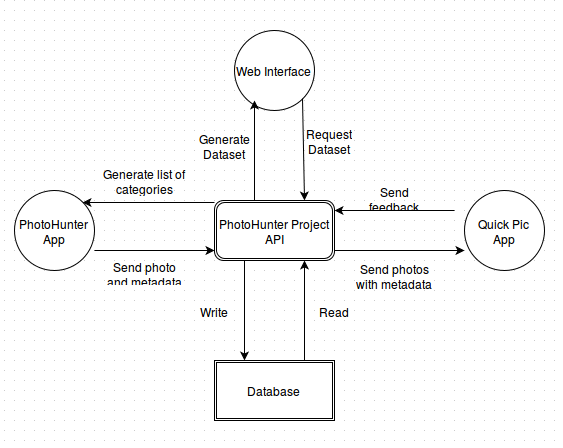
\includegraphics[scale = 0.5]{ss_flowchart}
\end{figure}

\subsubsection{Researcher Interface}
The researcher interface allows users to request datasets, view the status of
any open dataset, and download their dataset.

\paragraph{Create Account}
The create account form allows a new user to register their information in the
database. The Go server generates an HTML form requesting the user's name,
email address, requested user name, and password. When the user submits the
form, the password is encrypted using bCrypt, a Go library, and all information
is added to the user table in the database.

\paragraph{Log in to Account}
The login form allows a user to log in to their account. Once a user inputs
their user name and password and submits, the Go server selects the user name
from the user SQL table, checks the provided password against the correct one,
and provides the user with an error message if the account can not be found. If
the log in is successful, a new session is created associated with the logged
in user.

\paragraph{Update Account}
The account page allows users to update their information. The user may
complete an HTML form requesting a new password or providing a new email
address. The user's information is then updated in the database.

\paragraph{Request Dataset}
The request dataset functionality allows a user to provide information about a
dataset they desire. When a user requests a new dataset, an HTML form is
provided allowing the user to specify their needs. The form requires the user
to describe the following about the dataset:
\begin{itemize}
  \item The subject material of the dataset
  \item The time of day that the photos should be taken
  \item The location that the photos should be taken
  \item The minimum number of photos needed for the dataset
\end{itemize}
If one of these properties is irrelevant to the user, then they may specify
that on the form as well. After the dataset is described, the user may submit
it to the database.

\paragraph{View Dataset Status}
The researcher interface also allows the user to view the status of their
datasets. When this page is viewed, the Go server provides the total count of
the photos that currently exist for the dataset.

\begin{figure}[H]
  \caption{Researcher Interface Mockup}
  \centering
  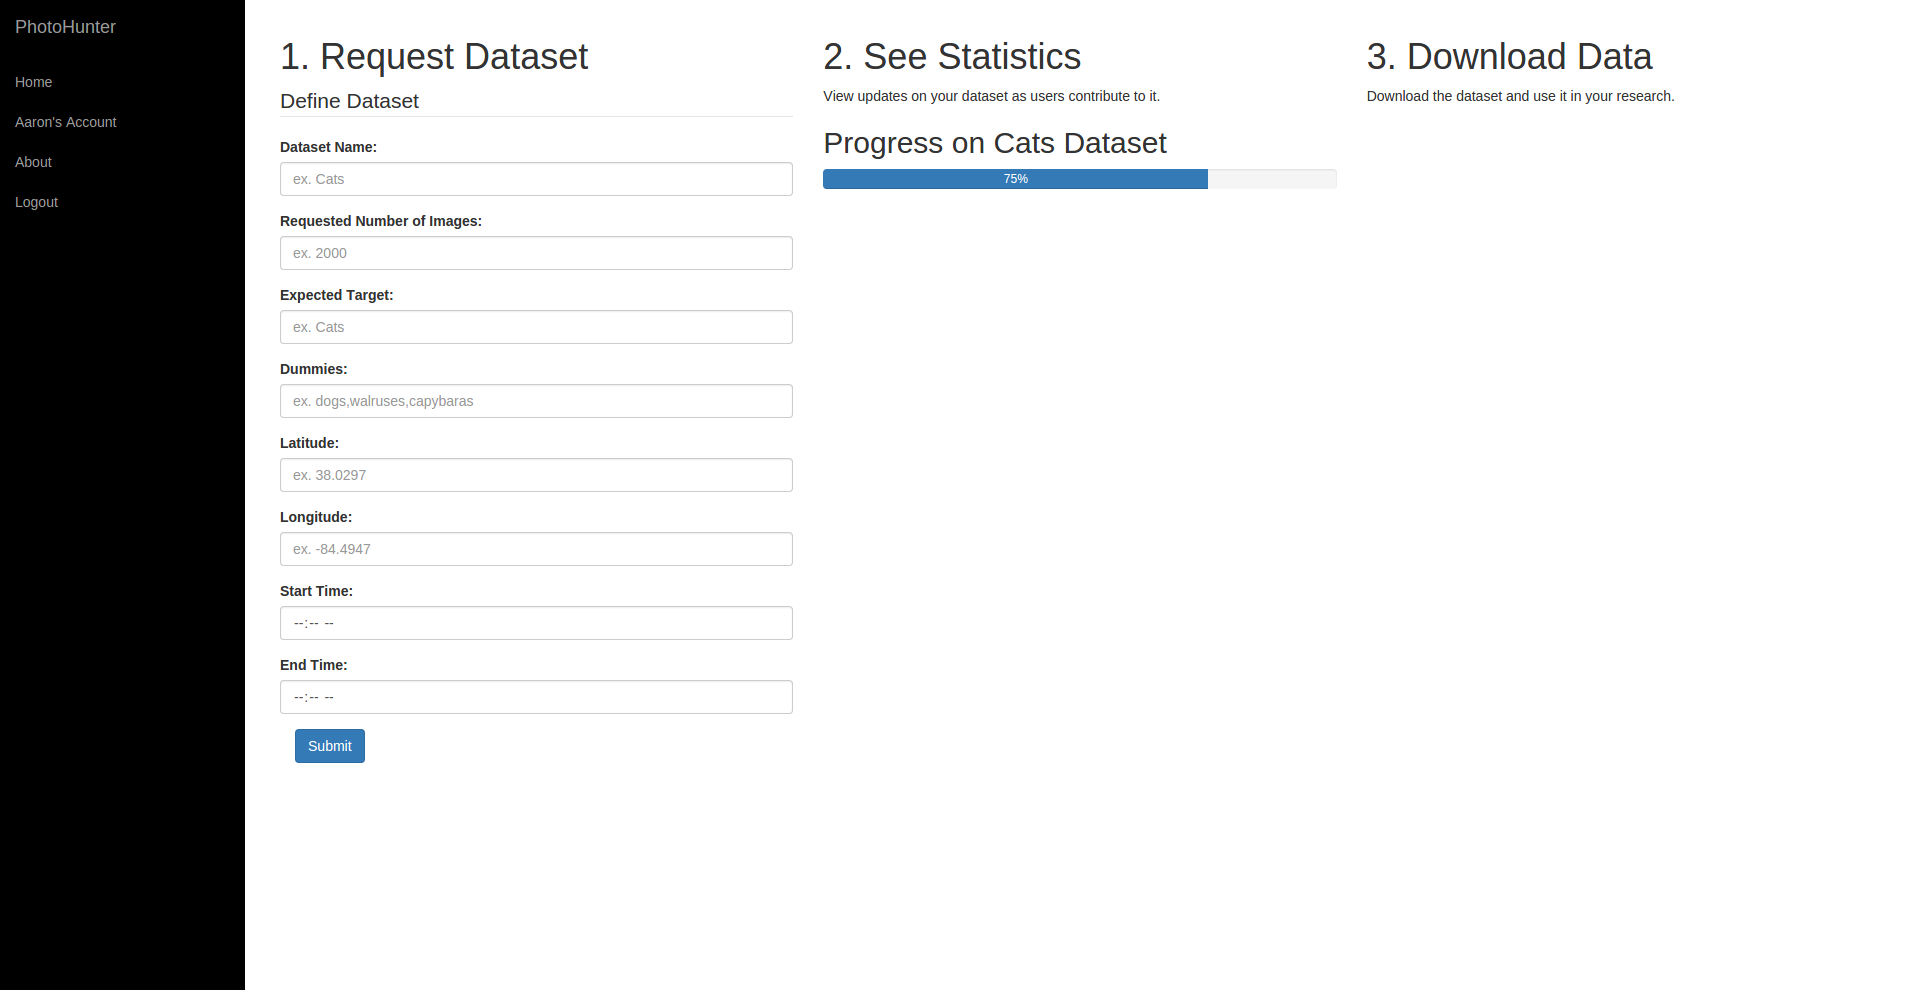
\includegraphics[width=\textwidth,height=\textheight,keepaspectratio]{researchers}
\end{figure}

\subsubsection{PhotoHunter}
The PhotoHunter application allows users to compete against one another to
capture photos in a scavenger hunt.

\paragraph{Create Account/Logging In}
The PhotoHunter application will use a Facebook API to allow users to create
accounts and log in using their Facebook accounts.

\paragraph{Provide Lists}
When a user is logged in, the application gets their location data. This data
is sent to the PhotoHunter API, which then provides a list of subjects for user
to photograph.

\paragraph{Select Topic and Photograph}
The user may choose a topic from the list of available ones. Their smart
phone's camera is then opened. After the user takes a photo and confirms it,
the application uploads the photo the database. The user's points are then
updated in the database.

\begin{figure}
  \centering
  \begin{subfigure}[b]{0.49\textwidth}
    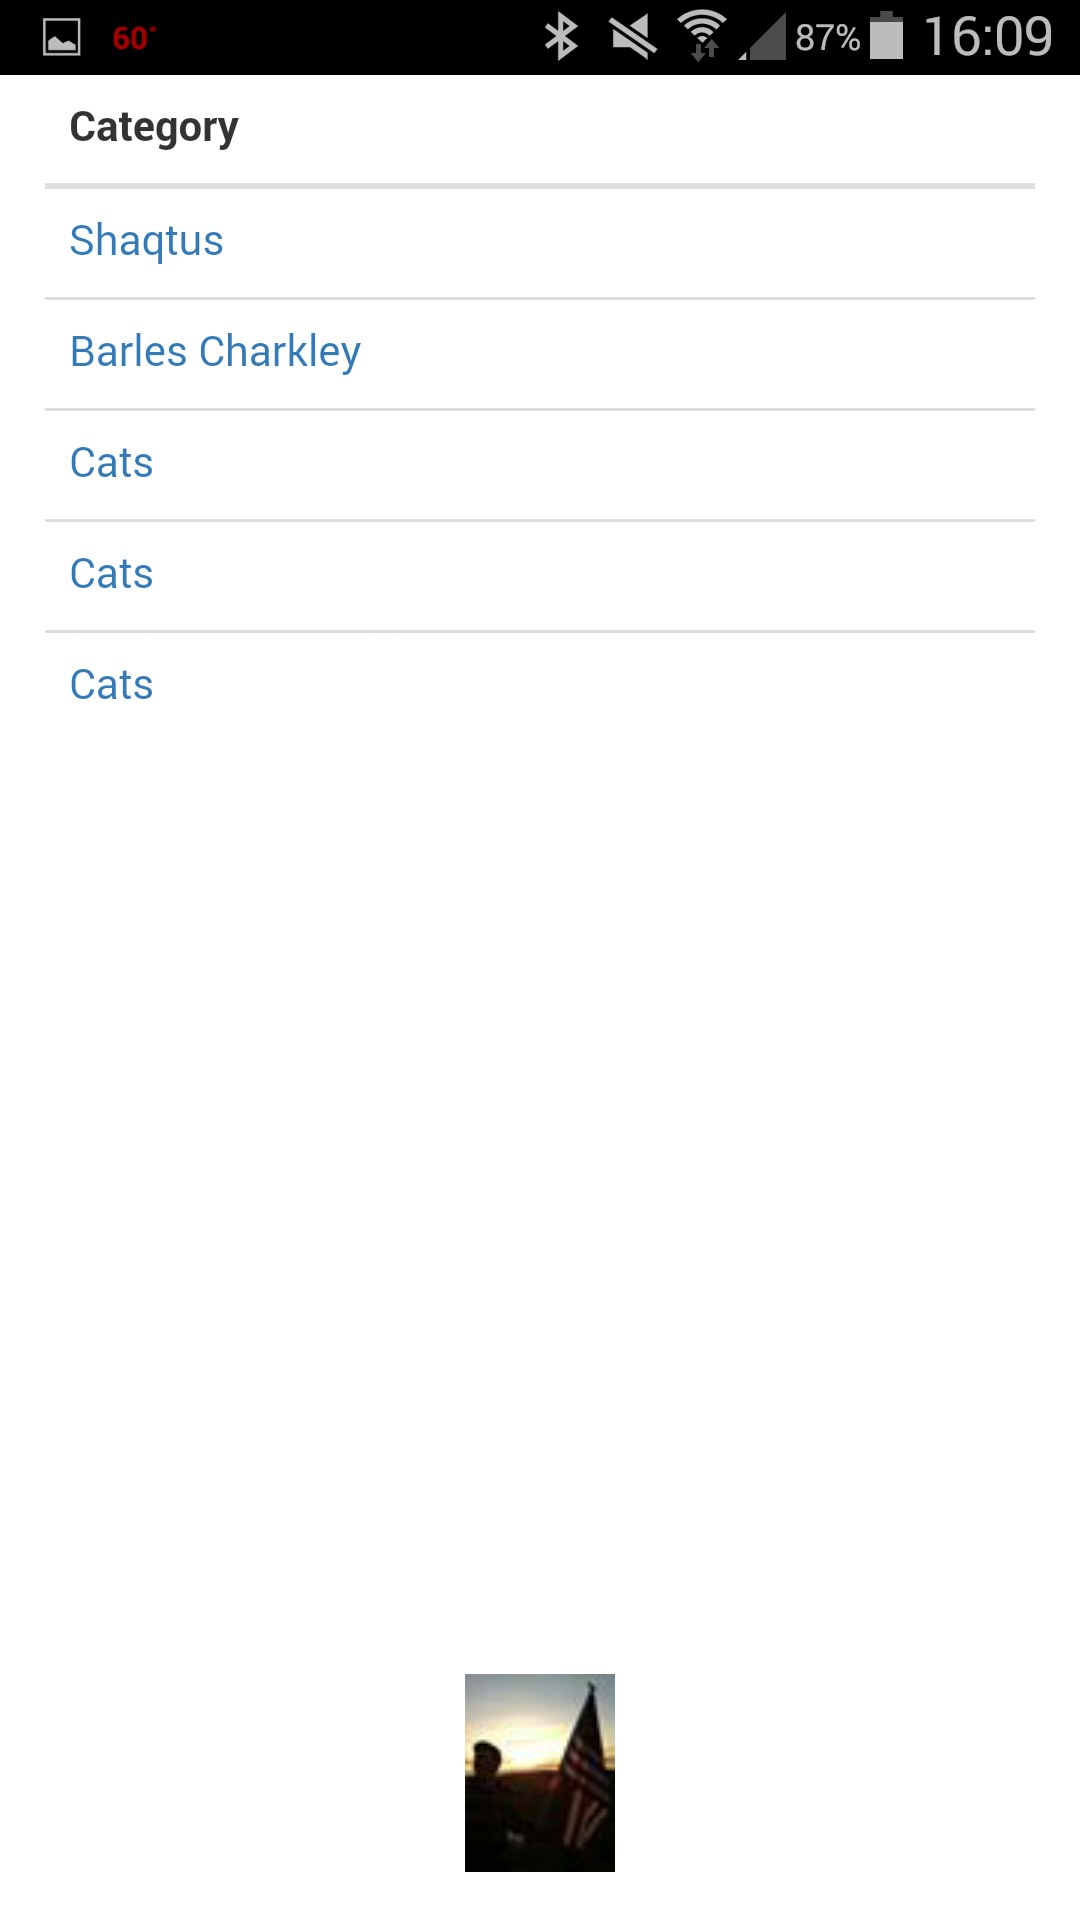
\includegraphics[width=\textwidth]{photohunter/list}
    \caption{PhotoHunter Scavenger List Mockup}
  \end{subfigure}
  \begin{subfigure}[b]{0.49\textwidth}
    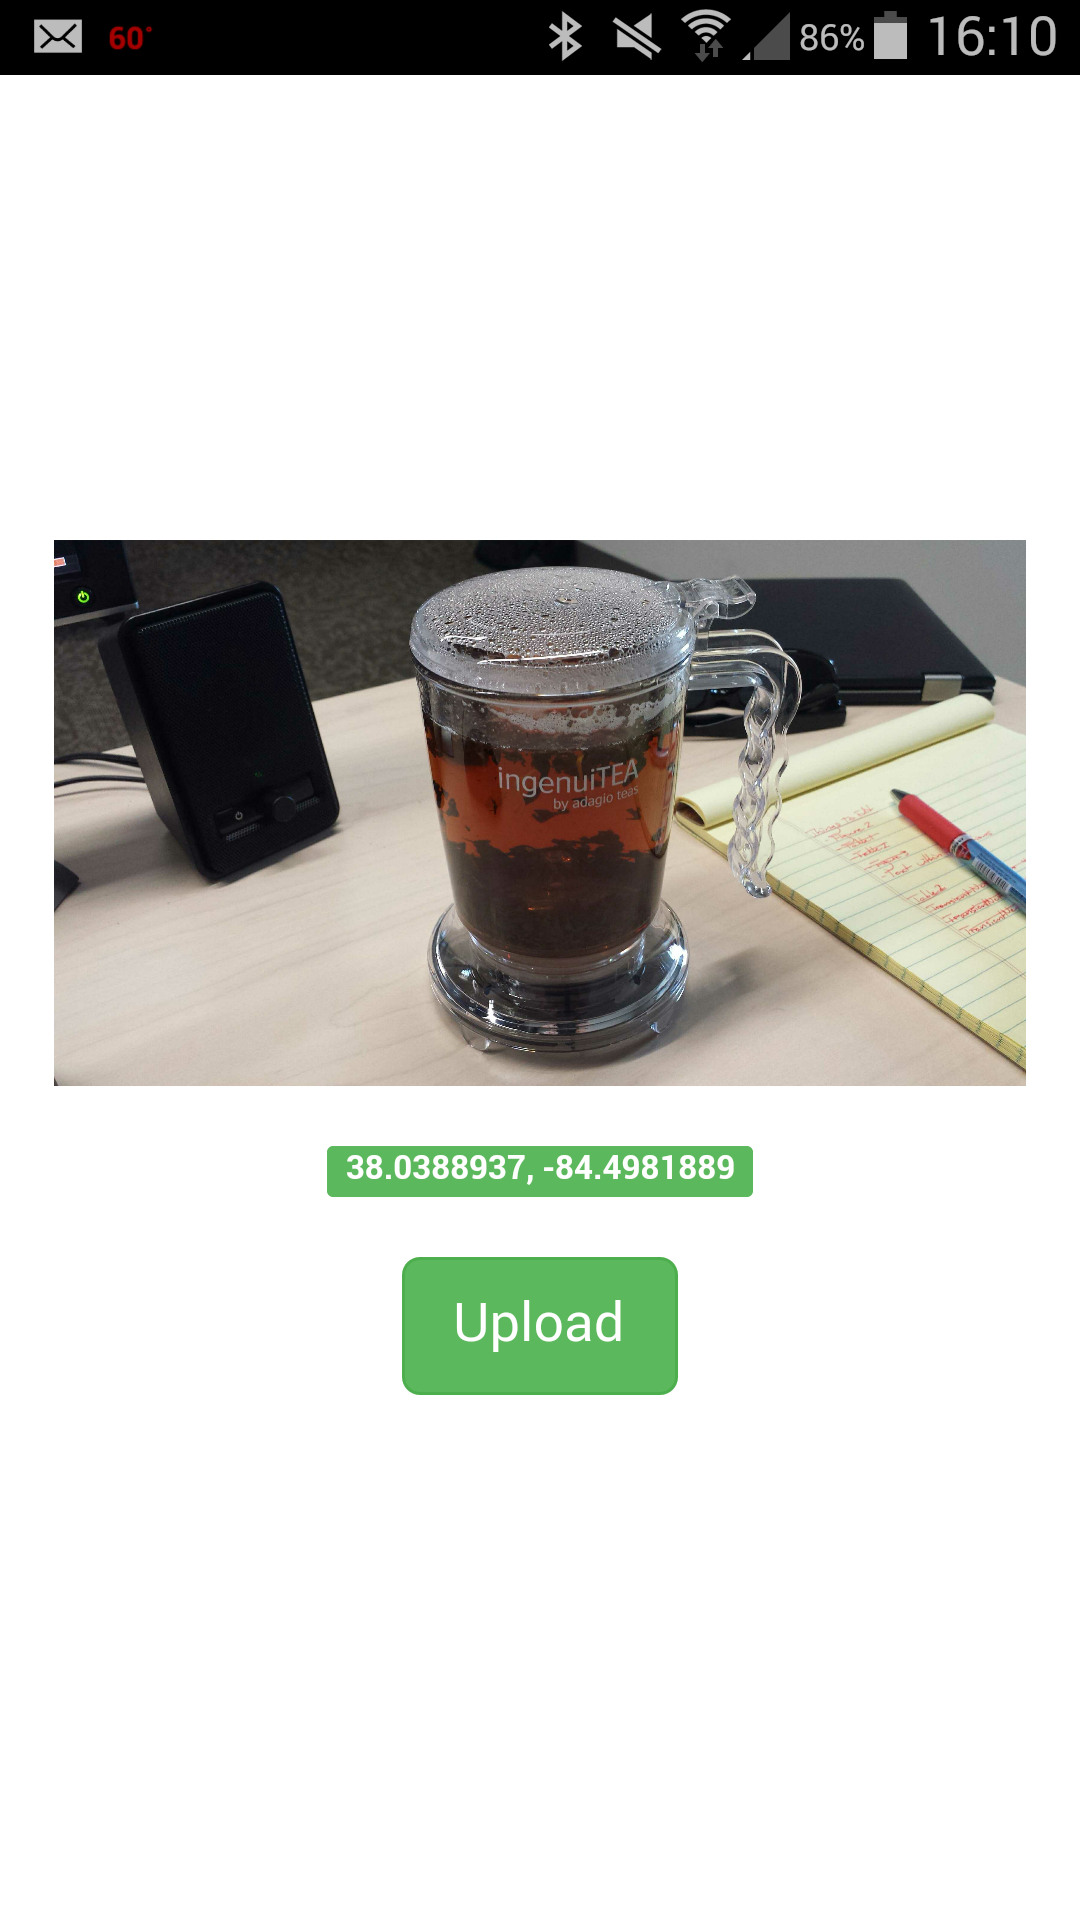
\includegraphics[width=\textwidth]{photohunter/submit}
    \caption{Photohunter Upload Mockup}
  \end{subfigure}
\end{figure}

\subsubsection{QuickPic}
The QuickPic application allows users to compete against one another by
quickly identifying the subjects of images.

\paragraph{Create Account/Logging In}
The QuickPic application will use a Facebook API to allow users to create
accounts and log in using their Facebook accounts.

\paragraph{Quiz}
When a user has logged in, they may begin a quiz. The quiz takes images from
the database that were submitted by the PhotoHunter application, and generates
four choices. One of these choices is the expected subject, based on the
dataset that the image was submitted to in PhotoHunter. The application shows
the user the image for a brief second, then asks the user to choose the correct
label. The user's answer is then submitted to the database. The user then
receives a number of points based on the answers given by other users.

\begin{figure}
  \centering
  \begin{subfigure}[b]{0.49\textwidth}
    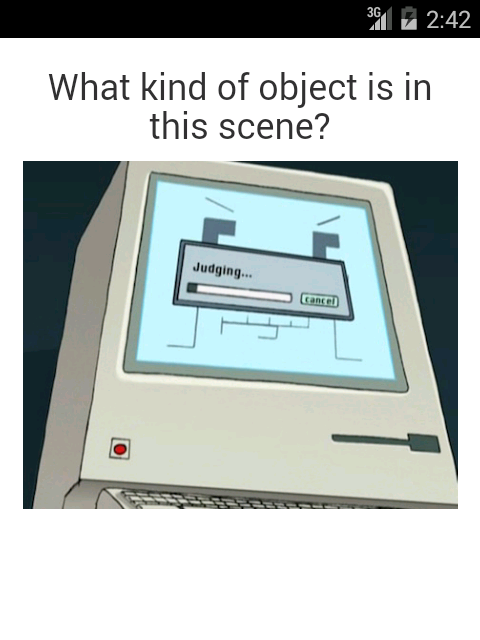
\includegraphics[width=\textwidth]{ss_quickpic_image}
    \caption{QuickPic Image Mockup}
  \end{subfigure}
  \begin{subfigure}[b]{0.49\textwidth}
    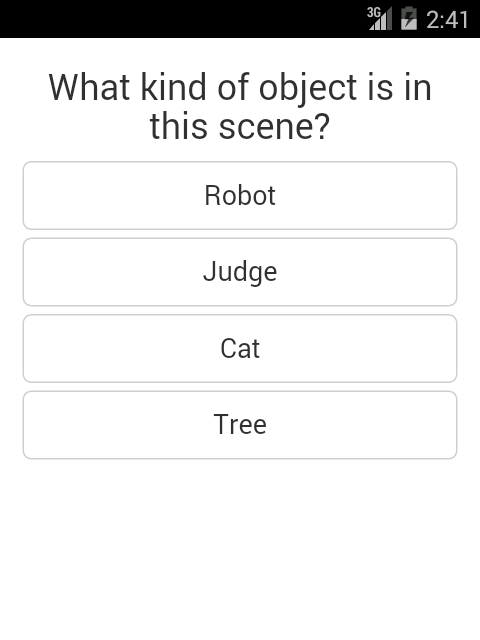
\includegraphics[width=\textwidth]{ss_quickpic_options}
    \caption{QuickPic Options Mockup}
  \end{subfigure}
\end{figure}

\subsection{API}

\paragraph{Create Dataset from Request}

Members of Research Teams (RTs) will provide Requests, which describe
the kind of data the RTs are looking for.  The internals of the API will
generate PhotoHunter and QuickPic jobs to collect data for the
Requests.

\paragraph{Generate Scavenger Lists for PhotoHunter}

Scavenger Lists are the jobs generated for PhotoHunter.  For a given
Request, one scavenger list entry for each requirement presented in
the request. For example, if the RT requests the following dataset:

\begin{itemize}
  \item Cats or Dogs
  \item Between 1pm and 8pm EST
\end{itemize}

Then the API will generate the following scavenger list entries:

\begin{itemize}
  \item Dogs Between 1pm and 8pm EST
  \item Cats Between 1pm and 8pm EST
\end{itemize}

The Request is expected to already have the data laid out in such a manner that
constructing this list is trivial (essentially the cartesian product of
elements of lists).

These Scavenger Lists will be made available to the PhotoHunter application
with some constraints.  The constraints are to be designed to avoid presenting
users with entries that are infeasible for them to complete.  The initial set
of constraints is:

\begin{itemize}
  \item Do not show users entries for which they are spatially ineligible (ie RT
    requests images from New York City, but user is in New Hampshire)
  \item Do not show users entries for which the non-repeating time requirement
    has already passed (example: RT requests images for the month of February,
    2015, but it is now March, 2015)
\end{itemize}

More constraints may be added based on further brainstorming, development and
testing with input from the customer.

\paragraph{Add Photo to Dataset}

When a Scavenger List entry is completed by a user of the PhotoHunter
application, a Photo is submitted to the API.  The API will store the Photo in
a database, along with both the dataset it was captured for and the entry that
the user claimed it matched.  This information with be available to the
requesting RT.

\paragraph{Get Photo and Labels for QuickPic}

The QuickPic application will request Photo and Label data from the API at a
rate of 1 Photo at a time.  Each response will include the Photo and 4 Labels.
The set of Labels will include:

\begin{itemize}
  \item The Label claimed by the user who submitted the photo via PhotoHunter
  \item The most popular Label according to QuickPic votes
\end{itemize}

The remaining Labels will be randomly chosen.  If the two required Labels are
the same, then there may be 3 random Labels chosen.

\paragraph{Calculate Points for Both Applications}

Points will be calculated in the following manner:

\begin{itemize}
  \item A base amount (say, 10) is always given simply for completing a task.
  \item Further points may be awarded based on confidence in the choice's
    accuracy.  Accuracy will be determined by comparing to the histogram of
    choices made by other users.  The number of additional points awarded will
    be $90 \times$ Confidence, where Confidence is on the range of
    $[0, 1]$.

  \item Points will be back-propagated to the PhotoHunter application at a rate
    of 1 PhotoHunter point per 10 QuickPic points.  This lowered rate was
    chosen because for each Photo, 1 PhotoHunter user may receive points but
    arbitrarily many QuickPic users may receive points.
\end{itemize}

\textbf{Note: The values of points and rates are subject to change based on
  testing and input from the customer.  These are not necessarily the final
values.}

\paragraph{Analyze QuickPic Label Choices}

Label choices from QuickPic will be analyzed using as-of-yet undetermined
statistical methods to determine what the probably True Label is and the
confidence on the Claimed Label.  Information about the choices will be made
available to the Research Teams receiving the images and labels.

The output from this method is important for the \textit{Calculate Points for
Both Applications} stage.

\subsubsection{ER Diagram}

See Figure \ref{er}.

\begin{figure}
  \centering
  \includegraphics[width=\textwidth]{er}
  \caption{ER Diagram}
  \label{er}
\end{figure}

\subsection{Use Cases}
\subsubsection{Researcher Interface}
When visiting the researcher interface, a user may do one of the following:
\begin{itemize}
  \item Log In: A user can log in to their account using their credentials. They will then be taken to their dashboard.
  \item Create Account: A new user may create an account by signing up.
\end{itemize}

After logging in, a user may visit one of the following pages on the dashboard:
\begin{itemize}
  \item Datasets: This page is where the user may do any of the following:
    \begin{itemize}
      \item Request Dataset: A user may complete an HTML form specifying a
            dataset that meets their needs. The user may then submit the dataset definition
            to the database.
      \item View Datasets: A user may view the status of their datasets. As new
            images are submitted, verified, and added to the dataset, the updated number
            may be viewed by the researcher.
      \item Download Dataset: After a dataset is complete, a user may download their dataset.
    \end{itemize}
  \item Account: This page allows users to update account information,
        including their email address or password.

\end{itemize}
\subsubsection{PhotoHunter}

\begin{itemize}
  \item Log In: A user can log in to their account using their credentials.
        They will then be taken to their dashboard.
  \item Create Account: A new user may create an account by signing up.
\end{itemize}

After logging in, a user may visit one of the following views:

\begin{itemize}
  \item Scavenger List: A list of Scavenger List Entries which have been
        requested by Research Teams. Choosing an entry will launch the native Camera
        application, allowing users to capture and submit a picture.
  \item Account: A view allowing the user to update account information.
\end{itemize}

\subsubsection{QuickPic}

\begin{itemize}
  \item Log In: A user can log in to their account using their credentials. They will then be taken to their dashboard.
  \item Create Account: A new user may create an account by signing up.
\end{itemize}

\begin{itemize}
  \item Label Images: A user will be presented with an image to label.  The
    amount of time they are given to view the image may depend on their overall
    score.  They will then be asked to choose a label.  Upon choosing a label,
    they will be presented with some information about their accuracy and asked
    to label another image.
  \item Account: A view allowing the user to update account information.
\end{itemize}
\subsection{Design Considerations}
Initially, the mobile applications for the PhotoHunter Project were to be
developed for both iOS and Android. However, due to the limited time available
and scope of the project, the team decided to develop the applications just for
Android.



\section{Implementation}
Talk about how we implemented everything.

\section{Future Enhancements/Maintenance}
Currently, due to unforeseen issues with interfacing between Go and PostgreSQL, the coordinates for locations are stored as float values, instead of the GeoPoint type offered by PostGIS. This is due to the lack of support for array types in the Go PostgreSQL library. In the future, it would be preferable to switch these coordinates to the GeoPoint type, as it would allow greater functionality.\\

The team would also like to implement leaderboards and a versatile point system for the two mobile applications. This functionality was pushed to the future due to time constraints. \\

As the applications are further developed, the team would like to market them and deploy to other platforms, such as iOS. The applications were developed in Cordova to simplify the process of iOS development. To increase marketability, the applications would be further "gameified." As usage of the system increases, an more robust security system would need to be implemented as well.

\section{Conclusions}

One of the important lessons we learned this semester is that learning new
framework and tech greatly slows the progress of development. None of us were
familiar with Cordova and the most knowledgeable of us was only barely familiar
with mobile app development. Further, we had not built any web APIs in Go
before and had no experience working with PostgreSQL extensions. However, once
we overcame the learning curves, we were pleased with the technology choices we
made.

We also learned how difficult it is to navigate an API with confusing and
inconsistent documentation. In our case, the culprit was the Facebook Login
API.\@ We ultimately succeeded, but not before many hours were spent figuring out
what is a simple process explained poorly.

As mentioned above, we were very pleased overall with our technology
choices. We would not change any of those at this time. Given the opportunity
to begin the semester again, we would like to have laid out a clear schedule
with milestones sooner in the project lifetime. Confusion about what needed to
be done when impacted our progress early in the semester, although we
ultimately got that sorted out. One thing that we would also change is the
order in which features were completed. We completed the database, QuickPic,
PhotoHunter and the Research Interface --- but not the API tying them
together. It would have been better to have a fully working API than a second
application that could only partially interact with the backend.

Both our customer and our team consider our project reasonably successful. We
did not complete all objectives. However, we made good progress and laid the
groundwork for future development.

\section{References}
Cite everything we used.
\begin{enumerate}

\item \textbf{Apache Cordova:} \url{https://cordova.apache.org/}
\item \textbf{Golang:} \url{https://golang.org/}
\item \textbf{PostgreSQL:} \url{http://www.postgresql.org/}
\item \textbf{PostGIS:} \url{http://postgis.net/}
\item \textbf{Phonegap Facebook Plugin:} \url{https://github.com/Wizcorp/phonegap-facebook-plugin}
\item \textbf{PQ Library for Go:} \url{https://github.com/lib/pq}
\item \textbf{Gorilla Sessions for Go:} \url{http://www.gorillatoolkit.org/pkg/sessions}
\item \textbf{Bootstrap:} \url{http://getbootstrap.com/}

\end{enumerate}

\section{User's Manual and Installation Guide}
\subsection{PhotoHunter}
The PhotoHunter application can be installed by downloading the apk file to an
Android device (Version 4.4.2) and installing it through the phone's interface.
Upon launch, the app will display the title screen with a log in button.
Clicking the login button will prompt the user to login using their Facebook
credentials.  Once logged in, the user is presented with a list of categories
to choose from, as well as a button (their Facebook profile picture) linking to
their account page.  Clicking on the profile picture button sends the user to a
page with their account information, filled out using the Facebook API.
Clicking on a category in the category list sends the user to a photo capture
page.  Clicking the capture button opens the native camera application on the
user's phone and allows the user to take a picture.  Once the picture is taken,
an upload button and the user's location appear.  Clicking on the upload button
sends the image to the database.

\subsection{QuickPic}

The QuickPic application can be installed by downloading the apk file to an
Android device (Version 4.4.2) and installing it through the phone's
interface. Upon launch, the app will display the title screen with a log in
button. Clicking the log in button will prompt the user to log in with their
Facebook account.

Once logged in, the user is presented with the main menu. Three buttons are
displayed: Photo Quiz, Statistics, and Leaderboards. However, only the 'Photo
Quiz' button is implemented at this time. Clicking this button will begin a
photo quiz. An image will be displayed for a very short period (presently
750ms), and then a list of potential categories will be presented to the
user. Upon selecting a category, statistics about the distribution of category
choices are presented. This statistics screen has two buttons: Menu and
Continue. Menu returns to the main menu, and Continue presents the user with
another image.

\subsection{Researcher's Interface}

\end{document}
